\documentclass[10pt,journal]{IEEEtran}\usepackage{longtable}
\usepackage{graphicx} 
\usepackage{sidecap}
\usepackage{balance}
\usepackage{amsmath}
%\usepackage{cite}
\usepackage{amssymb}
\usepackage{amssymb}
\newcommand*{\QEDA}{\hfill\ensuremath{\blacksquare}}%
\newcommand*{\QEDB}{\hfill\ensuremath{\square}}%
\usepackage{siunitx}
\usepackage[none]{hyphenat}
\usepackage[margin=0.7in]{geometry}
\usepackage{esvect}
\usepackage{braket}
\usepackage{listings}
\usepackage{epstopdf}
\usepackage{subfigure}
\usepackage{color} %red, green, blue, yellow, cyan, magenta, black, white
\usepackage{verbatim}
\usepackage{mwe}
\usepackage{array}
\newcolumntype{$}{>{\global\let\currentrowstyle\relax}}
\newcolumntype{^}{>{\currentrowstyle}}
\newcommand{\rowstyle}[1]{\gdef\currentrowstyle{#1}%
  #1\ignorespaces
}
\usepackage{hhline}
\definecolor{mygreen}{RGB}{28,172,0} % color values Red, Green, Blue
\definecolor{mylilas}{RGB}{170,55,241}
\graphicspath{{Figures/}}
\DeclareSIUnit\uvrms{\micro\volt{}_{RMS}}
\DeclareSIUnit\mvrms{\milli\volt{}_{RMS}}

\begin{document}
\lstset{language=Matlab,%
    %basicstyle=\color{red},
    breaklines=true,%
    morekeywords={matlab2tikz},
    keywordstyle=\color{blue},%
    morekeywords=[2]{1}, keywordstyle=[2]{\color{black}},
    identifierstyle=\color{black},%
    stringstyle=\color{mylilas},
    commentstyle=\color{mygreen},%
    showstringspaces=false,%without this there will be a symbol in the places where there is a space
    numbers=left,%
    numberstyle={\tiny \color{black}},% size of the numbers
    numbersep=9pt, % this defines how far the numbers are from the text
    emph=[1]{for,end,break},emphstyle=[1]\color{red}, %some words to emphasise
    %emph=[2]{word1,word2}, emphstyle=[2]{style},    
}




%%%%%%%%%%%%%%%%%%%%%%%%%%%%%%%%%%%%%%%%%%%%%%%%%%%%%%%%%%%%%%%%%%%%%%%%%%%%%%%%%%%%%%%%%%
\title{EE 315\\Final Project}
\author{Thomas Flores and Samuel Lenius}
\date{\today}
\maketitle
%%%%%%%%%%%%%%%%%%%%%%%%%%%%%%%%%%%%%%%%%%%%%%%%%%%%%%%%%%%%%%%%%%%%%%%%%%%%%%%%%%%%%%%%%%

%%%%%% ABSTRACT %%%%%%%
\begin{abstract}
\lipsum[1]
\end{abstract}
%%%%%%%%%%%%%%%%%%%%%


%%%%%%% INTRODUCTION %%%%%%%%%%
\section{Introduction}
\begin{figure}[b]
\begin{center}
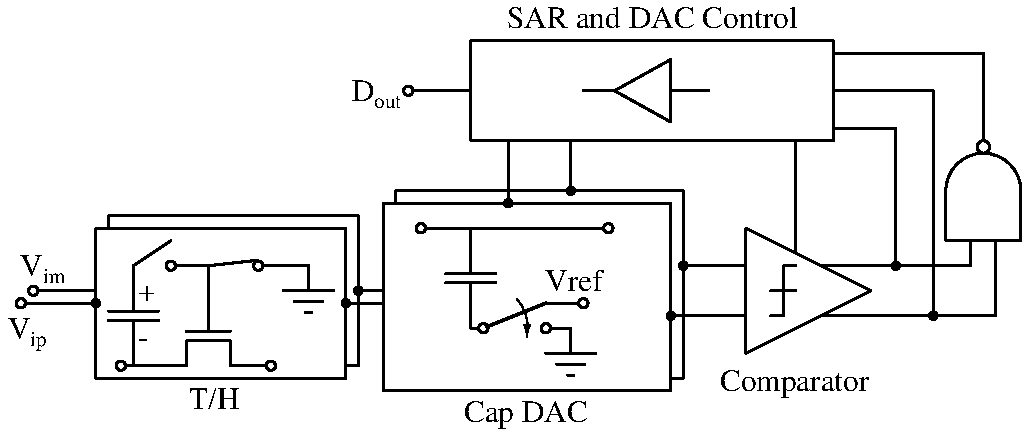
\includegraphics[width=1\columnwidth]{TopLevel.pdf}
\caption{Top level design for a fully differential asynchronous SAR ADC.}
\label{fig:TopLevel}
\end{center}
\end{figure}
\lipsum[1-3]
%%%%%%%%%%%%%%%%%%%%%%%%%%%%

\section{Block Design}
%%%%%%% COMPARATOR DESIGN %%%%%%%%%%%%
\subsection{Comparator}
\begin{figure}[tb]
\begin{center}
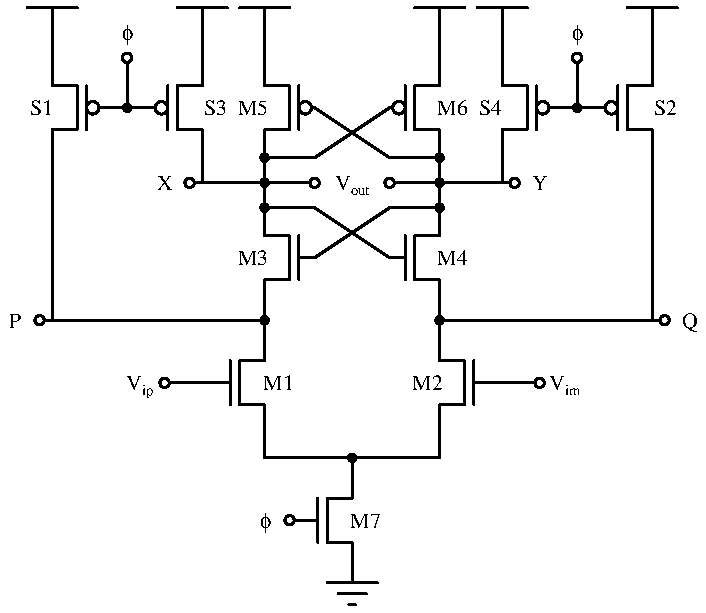
\includegraphics[width=1\columnwidth]{StrongArmLatch.pdf}
\caption{Circuit topology for the strong arm latch comparator.}
\label{fig:StrongArmLatch}
\end{center}
\end{figure}
Proper optimization of the comparator element in the SAR ADC will provide the greatest improvement in our figure of merit, as it will ultimately set the maximum speed of our design. Given that our figure of merit is proportional to the power consumed for each decision, the ideal design includes a dynamic comparator which only draws current during the decision time. For this reason, we choose the Strong Arm Latch (Figure \ref{fig:StrongArmLatch}) for its energy efficiency and simple design \cite{Razavi:bp}.

To size our comparator to first order, we begin by considering the required noise specification of the total SAR ADC. We can derive the maximum noise power for our full-scale signal power as
\begin{equation}
\sigma_{n,in}^2=\frac{P_{sig}}{10^{SNR_{spec}/10}}=\frac{\frac{\left(0.5V_{FS}\right)^2}{2}}{10^{\frac{SNR_{spec}}{10}}}
\end{equation}
Because we are designing to first order and want to budget a large amount of noise to the comparator function to improve speed, we impose a slightly higher noise spec of \SI{58}{\decibel}, thereby allocating half of our noise budget to the comparator. This gives an input referred noise requirement of $\sigma_{n,in}=\SI{445}{\uvrms}$ for $V_{FS}=\SI{1}{\volt}$.

We approximate the input referred noise for the strong arm latch as
\begin{equation}
\sigma_{n,in}^2\approx\frac{8\gamma}{A_v}\frac{kT}{C_{P,Q}}
\label{eq:InputNoise}
\end{equation}
where the gain $A_v$ during the amplification phase can be approximated as
\begin{equation}
A_v\approx\frac{g_{m1,2}}{I_D}V_{tn}
\label{eq:StrongArmGain}
\end{equation}
We select $\frac{g_m}{I_D}=15$ as this provides a reasonable tradeoff between speed and power of the transistor. From simulations, we find that the approximate threshold voltage $V_{tn}\approx\SI{300}{\milli\volt}$ for our nmos devices. We can then solve for the minimum capacitance necessary nodes P and Q using Equations \ref{eq:InputNoise}, \ref{eq:StrongArmGain}, and $\sigma_{n,in}=\SI{500}{\uvrms}$ 
\begin{equation}
C_{P,Q}\geq\frac{8\gamma}{A_v}\frac{kT}{\sigma_{n,in}^2}\rightarrow C_{P,Q}\geq\SI{31.11}{\femto\farad}
\end{equation}

To begin our design, we create a unit comparator constructed from some reasonable design choices. To maximize speed in the cross coupled inverters, we assume that pmos elements M5,6 should be twice the width of the nmos elements M3,4. To size M3,4, we must limit the widths so they do not significantly contribute to the mismatch at the input. For our design with $A_v\approx4$, this means that $W3,4\geq\frac{1}{4}W1,2$ due to the offset referral to the input. M7 must be able to bias the complete latch structure, and so we set $W7=2W1,2$. Finally, we size S1-S4 such that they are equal width to M1,2.

Our design methodology involves sweeping this unit cell over $W1$ until the $C_{P,Q}$ is above spec. A transient noise simulation is conducted to verify the input referred noise voltage over spec. The first order design resulted in much less input referred noise, and so the unit cell width W1 was decreased to approach the noise spec. The resulting sizing is shown in Table \ref{tbl:ComparatorDesign}.

\begin{table}[h]
\caption{Width sizing of strong arm latch comparator topology (\SI{}{\micro\metre}). All transistors minimum length $L=\SI{90}{\nano\metre}$}
\begin{center}
\begin{tabular}{c|c|c}
\hline \rowstyle{\bfseries} Transistor & \rowstyle{\bfseries} Unit & \rowstyle{\bfseries}  Optimized \\ \hline
M1,2 & \SI{1}{\micro\metre} & \SI{5.3}{\micro\metre} \\ \hline
M3,4 & $\frac{1}{4} W_{M1,2}$ & \SI{1.3}{\micro\metre}  \\ \hline
M5,6 & $2W_{M3,4}$ & \SI{2.6}{\micro\metre}\\ \hline
M7 & $2W_{M1,2}$ & \SI{10.6}{\micro\metre} \\ \hline
S1-4 & $W_{M1,2}$ & \SI{5.3}{\micro\metre}  \\ \hline
\end{tabular}
\end{center}
\label{tbl:ComparatorDesign}
\end{table}

%%%%%%%%%%%%%%%%%%%%%%%%%%%%%%%%%%


%%%%%%% BOOTSTRAPPED SWITCH DESIGN %%%%%%%%%%%%
\subsection{Track and Hold}
\begin{figure}[tbph]
\begin{center}
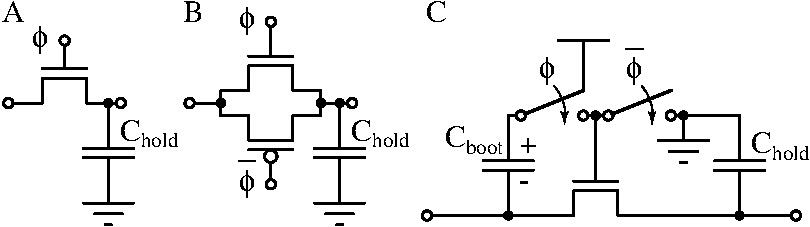
\includegraphics[width=1\columnwidth]{Switch_types.pdf}
\caption{Track and hold switch designs. A) Simple nmos swith, B) transmission gate, and C) bootstrapped nmos.}
\label{fig:SwitchTypes}
\end{center}
\end{figure}


For the SAR ADC to accurately reproduce the input signal in digital code, the signal must be relayed to the comparator input capacitors with minimal distortion. The initial sample acquisition, or "track" mode, must accurately follow the input and later hold the signal in "hold mode" on the comparator input capacitors for the SAR logic to determine the bit level. This requires the use of a switch with highly linear channel resistance across the input full-scale voltage. For a simple nmos switch (Figure \ref{fig:SwitchTypes}A), we can write the channel on resistance as
\begin{equation}
R_{on}=\frac{\mu_nC_{ox}\frac{W}{L}}{V_{DD}-V_{in}-V_{th}}
\label{eq:channel_res}
\end{equation}
where $V_g=V_{DD}$ and $V_{s}=V_{in}$. The on-resistance clearly shows a signal dependence $\propto\frac{1}{V_{in}}$, with the channel becoming infinitely resistive at $V_{in}=V_{DD}-V_{th}$. To alleviate this issue, a transmission gate can be used in which nmos and pmos devices with tied source and drain are driven out of phase (Figure \ref{fig:SwitchTypes}B), resulting in finite input resistance across all signal inputs due to the parallel combination of the channels. However, there remains strong signal dependence maximal around half of the full-scale, which will distort the signal. 

The transmission gate is also problematic due to input signal dependent charge injection incident upon the hold capacitor. The channel charge for the nmos device can be written as
\begin{equation}
Q_{ch}=WLC_{ox}\left(V_{DD}-V_{in}-V_{th}\right)
\label{eq:charge_inj}
\end{equation}
where $Q_{ch}\propto V_{in}$. 

For our track and hold circuit, we choose the bootstrapped nmos switch (Figure \ref{fig:SwitchTypes}C) for highly linear channel resistance. Equations \ref{eq:channel_res} and \ref{eq:charge_inj} indicate that signal dependence will be greatly reduced when $V_{gs}=V_{DD}-V_{in}$ is held constant. The bootstrapped nmos accomplishes this by maintaining a constant voltage drop of $V_{gs}=V_{DD}$ by connecting a precharged capacitor $C_3$ from the gate to source terminals. 
\begin{figure}[tbph]
\begin{center}
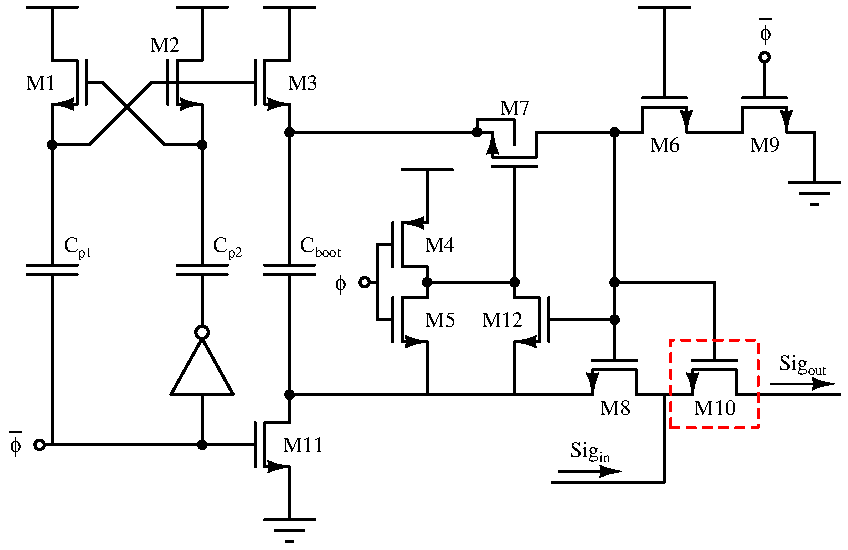
\includegraphics[width=1\columnwidth]{BootstrappedSwitch.pdf}
\caption{Circuit topology for the bootstrapped switch for improved on-resistance linearity and reduced charge injection. Switch M10 (red) denotes the main switch.}
\label{fig:BootstrappedSwitch}
\end{center}
\end{figure}
The complete circuit topology for the bootstrapped switch is shown in Figure \ref{fig:BootstrappedSwitch}. Here, M10 acts as the main nmos switch, with $C_{boot}$ connected across the gate and source terminals. The remaining switches work to precharge $C_{boot}$ and connect or disconnect it from M10 and discharge the M10 gate capacitance.

When $\phi=0$, $C_{boot}$ is disconnected from the  switch M10 by closing M7 and M8 and charged to the supply rail through M3 and charged to $V_{DD}$. During this time, the gate of M10 is tied to ground through M6 and M9. When $\phi=1$, M3 and M11 close, allowing $C_{boot}$ to be connected across M10 by opening M7 and closing M9. This allows the signal to pass through M10 while maintaining $V_{GS}=V_{DD}$. When $\phi=0$, $C_{boot}$ disconnects and recharges back to $V_{DD}$, while the gate capacitance of M10 is discharged to ground.

Sizing the bootstrapped switch is straightforward. The main design consideration involves the tradeoff between minimizing the on resistance by increasing width and minimizing charge injection by reducing width. 
We then considering the on resistance seen through the main switch M10 as
\begin{equation}
R_{on}=\frac{\mu_nC_{ox}\frac{W}{L}}{\frac{C_{par}}{C_{boot}+C_{par}}V_{DD}-\frac{C_{par}}{C_{boot}+C_{par}}V_{in}-V_{th}}
\end{equation}
To limit the signal dependence, we need to ensure $\frac{C_{par}}{C_{boot}+C_{par}}<1\rightarrow C_{boot}>C_{par}$ where $C_{par}$ is the parastitic capacitance as seen from the top plate of $C_{boot}$. As a design choice, we choose $C_{boot}>10C_{gM10}$, as the major capactive element in this path is the gate capacitance of the M10 switch. 

Sizing M3 and M11 remains the only critical choice. Here, the transistors must be large enough to ensure the capacitor charges completely to $V_{DD}$ within the sampling window. 

The remainder of the sizing is to ensure that the switches function as intended. M7 is sized large to ensure minimum resistance for the cap connection to the gate of M10. M4 and M5 are sized with reasonable widths such that $W_p=2W_n$, and M1 and M2 are equivalent. Finally, M6 and M9 are moderately sized to ensure fast discharge of the M10 gate capacitance. The resulting sizing of the bootstrapped topology is shown in Table \ref{tbl:BootstrappedDesign}.

\begin{table}[hb]
\caption{Sizing of bootstrapped switch topology. All transistors minimum length $L=\SI{90}{\nano\metre}$}
\begin{center}
\begin{tabular}{c|c}
\hline \rowstyle{\bfseries} Transistor & \rowstyle{\bfseries} Optimized  \\ \hline
M1 & \SI{1}{\micro\metre}  \\ \hline
M2 & \SI{1}{\micro\metre}  \\ \hline
M3 & \SI{2}{\micro\metre}  \\ \hline
M4 & \SI{2}{\micro\metre}  \\ \hline
M5 & \SI{1}{\micro\metre}  \\ \hline
M6 & \SI{5}{\micro\metre}  \\ \hline
M7 & \SI{10}{\micro\metre}  \\ \hline
M8 & \SI{5}{\micro\metre}  \\ \hline
M9 & \SI{5}{\micro\metre}  \\ \hline
M10 & \SI{25}{\micro\metre}  \\ \hline
M11 & \SI{2}{\micro\metre}  \\ \hline
M12 & \SI{1}{\micro\metre}  \\ \hline
$C_{boot}$ & \SI{300}{\femto\farad}  \\ \hline
$C_{p1}$ & \SI{200}{\femto\farad}  \\ \hline
$C_{p2}$ & \SI{200}{\femto\farad}  \\ \hline
\end{tabular}
\end{center}
\label{tbl:BootstrappedDesign}
\end{table}

%%%%%%%%%%%%%%%%%%%%%%%%%%%%%%%%%%



%%%%%%% DAC DESIGN %%%%%%%%%%%%
\subsection{9 Bit Capacitive DAC}

\begin{figure}[tbph]
\begin{center}
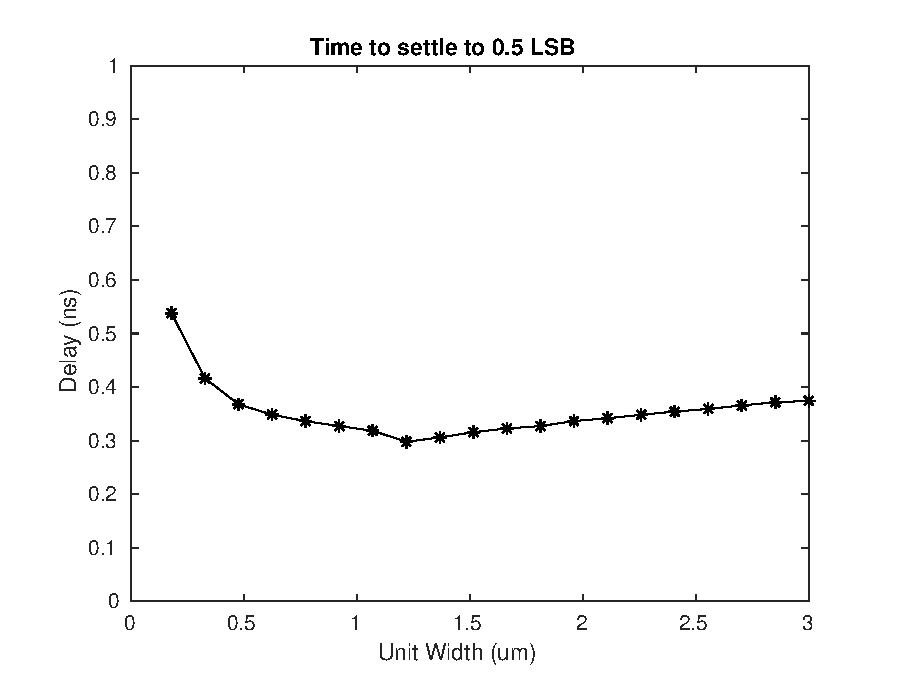
\includegraphics[width=1\columnwidth]{dac_optimization.eps}
\caption{Optimization of settling time vs device unit width.}
\label{fig:DacOptimization}
\end{center}
\end{figure}
\begin{figure}[tbph]
\begin{center}
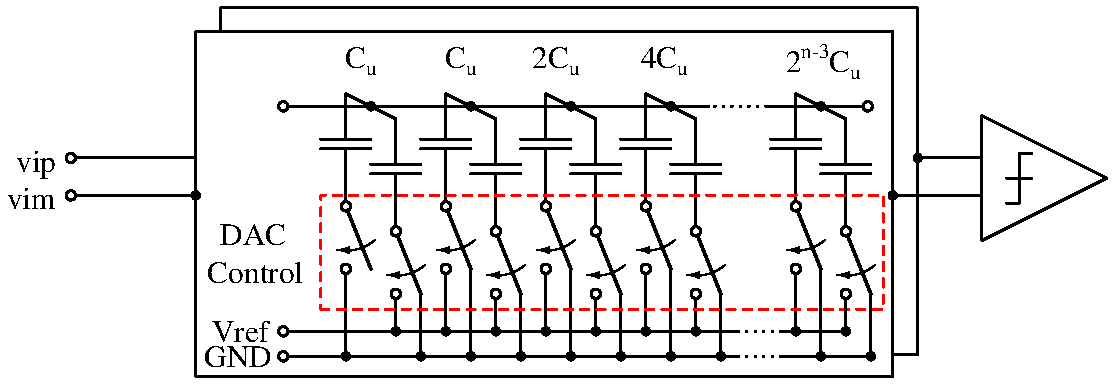
\includegraphics[width=1\columnwidth]{CapDacV3.pdf}
\caption{Capacitive DAC with top-plate sampling.}
\label{fig:CapDac}
\end{center}
\end{figure}

% TODO(sam) reference
Here we implement a 9 bit capacitive constant common mode top plate sampling DAC as in \cite{Tripathi:2013}.

Each bit of the DAC is binary weighted with a single dummy value in the
sequence 1, 1, 2, 4, 8, 16, 32, 64, 128.
For each bit there is both the top plate sampled capacitor and the corresponding inverter cell.

In order to have equal time constants between capacitors and inverter cells, equal scaling parameters are applied to each, hence the device widths of the cells follow the same sequence as the capacitors.

One complication of this approach is that the electrical effort to drive the inverters scales with this same sequence. 
Hence as the driver inverters scale up, the sequence of gate drive buffers must as well for optimal delay and power consumption.

This leads to each DAC inverter cell being designed individually for the expected range of electrical effort of that cell across optimization.

% TODO(sam) put a real circuit here
\begin{figure}[tbph]
\begin{center}
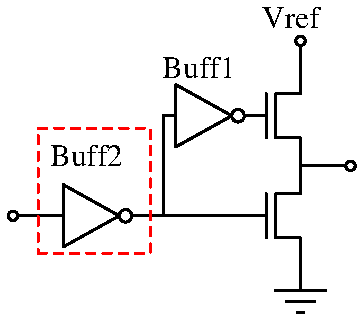
\includegraphics[width=1\columnwidth]{DAC_Switch.pdf}
\caption{DAC inverter unit cells.}
\label{fig:DACUnitInverterSch}
\end{center}
\end{figure}


% TODO(sam) reference
Our initial implementation of the inverter cell followed [2013 Tripathi] however we found that by using an inverter and a pair of N-channel devices we were able to achieve lower total delay and settling time. 

The specific issue with a standard inverter cell was that as the DAC switched it's MSB or MSB-1 bits, the dV/dT induced currents through the P-channel devices of the MSB-1 and MSB-2 cells caused a disturbance that reduced the gate overvoltage, hence increasing channel resistance and lengthening the duration of the glitch. 

By using a pair of N-channel devices we have applied a much higher gate overvoltage, and additionally the switching glitches now increase the gate overvoltage, improving the recovery time for glitches.
The use of two N channel devices here reduces the total gate capacitance to drive by a factor of two while reducing the output node parasitic capacitance, hence reducing DAC power overall.

Using a criterion of settling to within 1/2 LSB our optimized design has a delay of 370ps.
Accounting for the 1\% parasitic capacitance to ground on the top plate of the DAC capciators, our DAC reference voltage is 606mV in this design. 

%%%%%%%%%%%%%%%%%%%%%%%%%%%%%%%%%%



%%%%%%% LOGIC DESIGN %%%%%%%%%%%%
\subsection{Asynchronous Reset Logic}

\begin{figure}[tbph]
\begin{center}
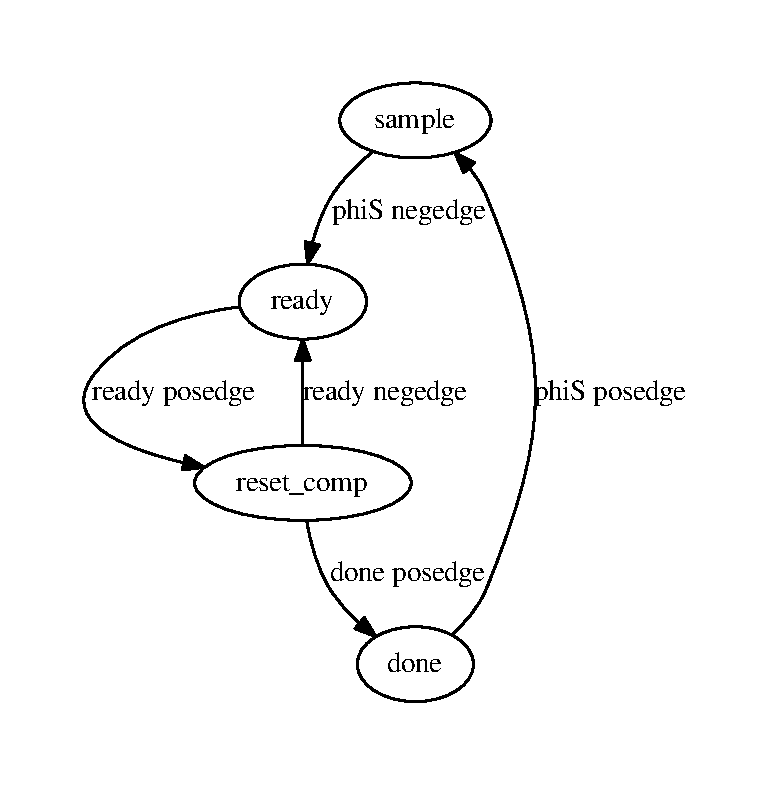
\includegraphics[width=1\columnwidth]{async.pdf}
\caption{State transition diagram for asynchronous reset logic.}
\label{fig:AsyncStateMachine}
\end{center}
\end{figure}

% TODO(sam) timing diagram

In this ADC we implement asynchronous reset logic as in \cite{Chen:2006}. The state machine that our asynchronous logic implements is as follows.

First the sampling clock edge rises, this opens the sampling gates and resets the internal state of the logic.

Second, the sampling clock drops and the asynchronous clock rises, enabling the dynamic comparator.

Third, the comparator makes a decision an one of it's two output lines drops. 
The outputs of the comparator are tied to the inputs of NAND gate as well as a buffer chain to drive the logic.
The reset state of the comparator has both lines high, hence the output of the NAND is low.
Once the comparator has made a decision, the output of the NAND is high, we call this signal 'Ready'. When Ready rises, we sample and shift one bit, and drop the asynchronous clock.

Fourth, after the bit is sampled, we reset the comparator. Here again we use the Ready signal to indicate that this step is finished. Once both of the comparator's output lines rise, the NAND's output will go to zero and we're prepared to convert the next bit. The Ready signal dropping will cause the clock to rise again, reenabling the comparator.

Fifth, once all 10 bits are shiftd out, we assert the done signal internally to the logic and the comparator is held in low power reset, ready for when the next sample comes in.

We compute the maximum synchronous sampling speed given our specifications for $P_{meta}$ and the measured performance characteristics of the circuit. Our comparator has a measured regeneration time of 16.7ps and a slewing time of 64ps. We require two FO4 buffers to connect our comparator to our SAR logic block, each with a delay of 40ps. Maximum synchronous sampling speed assuming a 50\% duty cycle clock, 12 clocks per conversion can be computed as follows:

\begin{equation}
  N_{taus} = ln\left(\frac{N_{codes}}{P_{meta}}\right) = 20.7
\end{equation}

\begin{equation}
  T_{clock,high} = N_{taus} * \tau_{comp} + 2 * T_{FO4} + T_{slew} = \SI{490}{\pico\second}
\end{equation}

\begin{equation}
  T_{clock} = 2 * T_{clock,high}
\end{equation}

\begin{equation}
  T_{sample,sync} = 12 * T_{clock}
\end{equation}

\begin{equation}
  F_{sample,sync} = \SI{85.1}{\mega\siemens\per\second}
\end{equation}

\cite{Chen:2006} gives us a speedup achievable for using asynchronous logic in equation 5 of that article. Here Chen shows that the expected speedup for an N bit converter approaches 2 for a large number of bits, for our 10 bit converter, the expected speedup is 1.56.
This means that for no additional energy per bit, that a converter using asynchronous logic can run over 1.5 times as fast as it's synchronous counterpart. The decision to use asynchronous logic here is obvious.

\begin{equation}
  F_{sample,async} = F_{sample,sync} * AsyncSpeedup = \SI{133.2}{\mega\siemens\per\second}
\end{equation}

This establishes the maximum achievable speed of our device while maintaining the $P_{meta}$ specification.


%%%%%%%%%%%%%%%%%%%%%%%%%%%%%%%%%%

%%%%%%% Results %%%%%%%%%%%%
\section{Results}
\subsection{Comparator}
\begin{figure}[tbph]
\begin{center}
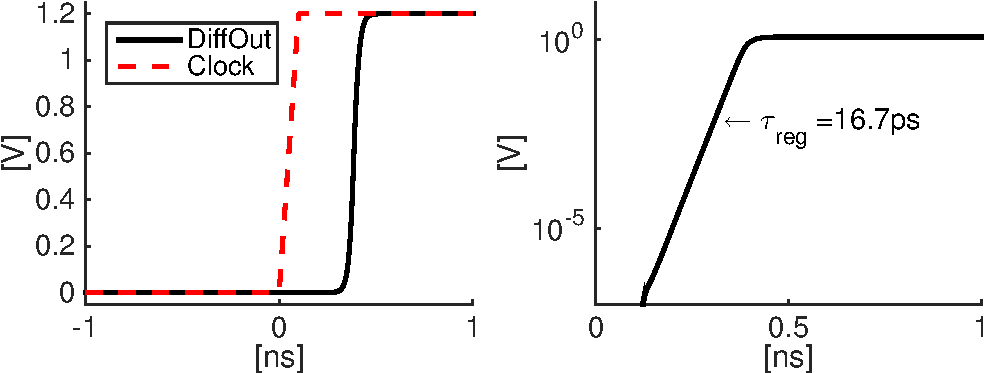
\includegraphics[width=1\columnwidth]{Comparator_Result_Reg_Time.pdf}
\caption{Comparator switching (left) and regeneration time (right).}
\label{fig:ComparatorRegTime}
\end{center}
\end{figure}
\begin{figure}[tbph]
\begin{center}
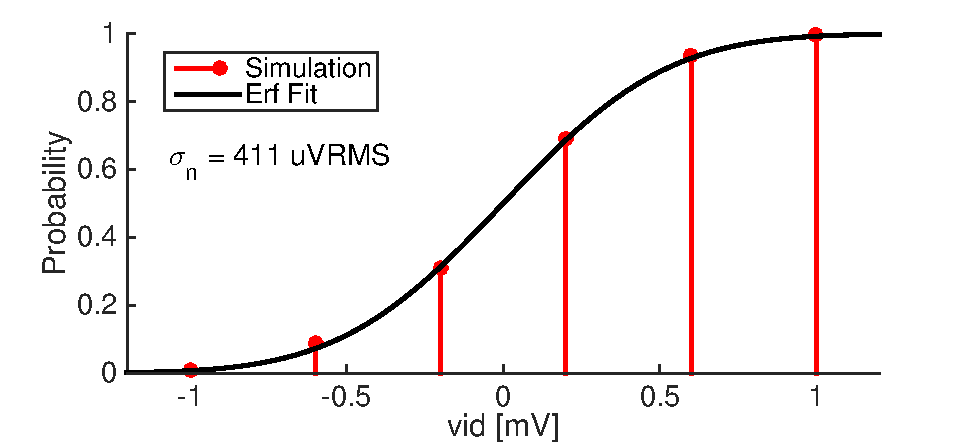
\includegraphics[width=1\columnwidth]{ComparatorTranNoise.pdf}
\caption{Transient noise simulation with varying input differential voltage. Error function fit extracts the input referred noise voltage $\sigma_{n}=\SI{411}{\uvrms}$}
\label{fig:ComparatorTranNoise}
\end{center}
\end{figure}
%%%%%%%%%%%%%%%%%%%%%%%%%%%%%%%%%%

%%%%%%% Conclusions %%%%%%%%%%%%
\section{Conclusions}
\lipsum[5]

%%%%%%%%%%%%%%%%%%%%%%%%%%%%%%%%%%



\bibliographystyle{IEEEtran}
\bibliography{IEEEabrv,References}
\end{document}


